\documentclass[journal,12pt,twocolumn]{IEEEtran}
\usepackage{graphicx}
\graphicspath{{./figs/}}{}
\usepackage{amsmath,amssymb,amsfonts,amsthm}
\newcommand{\myvec}[1]{\ensuremath{\begin{pmatrix}#1\end{pmatrix}}}
\usepackage{listings}
\usepackage{watermark}
\usepackage{titlesec}
\let\vec\mathbf

\titlespacing{\subsection}{0pt}{\parskip}{-3pt}
\titlespacing{\subsubsection}{0pt}{\parskip}{-\parskip}
\titlespacing{\paragraph}{0pt}{\parskip}{\parskip}
\newcommand{\figuremacro}[5]{
    
}
\lstset{
frame=single, 
breaklines=true,
columns=fullflexible
}
\thiswatermark{\centering \put(0,-105.0){
\includegraphics[scale=0.5]{iith.png}} }

\sloppy
\title{\mytitle}
\title{
Matrix Assignment - Conic
}
\author{Nikhil Nair}
\begin{document}
\maketitle
\tableofcontents
\bigskip


\section{\textbf{Problem}}
The minimum area of the triangle formed by the tangent to $\frac{x^2}{a^2}+ \frac{y^2}{b^2}=1$.\\


\section{\textbf{Solution}}
The equation of a conic is given as,  
\\

${\vec{x^{\top}V x} + 2\vec{u^{\top}x}} + f=0$
\\

where,
\\

$\vec{V}=\myvec{b^2&0\\ 0&a^2}$ and $\vec{u}=\myvec{0\\0}$
\\

for the given conic
\\

Let the point where the tangent touches the conic be $Q(acos\theta,bsin\theta)$
\\

Equation of tangent is given by,
\\

$\vec{(VQ +u)^{\top}}\vec{x} + \vec{u^{\top}Q} + f = 0$
\\
\\


$\vec{(VQ)}^{\top}\vec{x} = -f$
\\
\\
which can be written as 
\\

$\vec{n}^{\top}\vec{x} = C$
\\
\\

$n=\vec{VQ} = \myvec{ab^2cos\theta\\a^2bsin\theta}$ and $C=-f=(ab)^2$
\\

Since r and p are the intercepts on the x and y axis respectively
\\

$\vec{r}=\myvec{r\\0}$and $\vec{p}=\myvec{0\\p}$
\\

Now,
\\

$\therefore r=\frac{C}{\vec{n}^{\top}\vec{e_x}}$ and $p=\frac{C}{\vec{n}^{\top}\vec{e_y}}$
\\

where
\\
 
$ \vec{e_x}=\myvec{1\\0} $ and $\vec{e_y}=\myvec{0\\1}$
\\

are the units vectors on the x and y axis respectively
\\

Area of triangle is given by
\\  
\\$$\frac{1}{2} 
\begin{vmatrix}
       1&1&1\\\vec{o}&\vec{r}&\vec{p}
\end{vmatrix}$$
\vspace{0.6cm}

Area of triangle $$= \frac{1}{2} 
\begin{vmatrix}
       1&1&1\\0&r&0\\ 0&0&p
\end{vmatrix}$$
\\
\\

$\therefore$ Area = $\frac{1}{2}\frac{ab}{cos\theta sin\theta}$ = $
\frac{ab}{sin2\theta}$ 
\\
\\

Area will be minimum when $sin2\theta$ is maximum
\\
\\

Max. value of $sin2\theta = 1$
\\
\\

$\therefore$ Minimum area = ab  
\\
\\

The minimum area of the traingle formed by the tangent to the conic is $ab$
\\
\\

\section{\textbf{Verification using Gradient Descent}}

Using gradient descent method we can find minimum area of triangle\\ \vspace{2mm}
\begin{center}
$x_{n+1} = x_n - \alpha \nabla f(x_n)$ 
\\

\vspace{7mm}
$x_{n+1} = x_n + \alpha (2ab\frac{cos2\theta}{sin^2(2\theta)})$
\end{center}
\vspace{7mm}
Taking a=3, b=2, $x_0$=1,$\alpha$=0.001 and precision = 0.00000001, values obtained using python are:
\\
    
\begin{align}
        \boxed{\text{Minima} = 6}\\
        \boxed{\text{Minima Point} = 0.78}
\end{align}
\vspace{1mm}
\section{\textbf{Figure}}
\begin{figure}[h]
    \centering
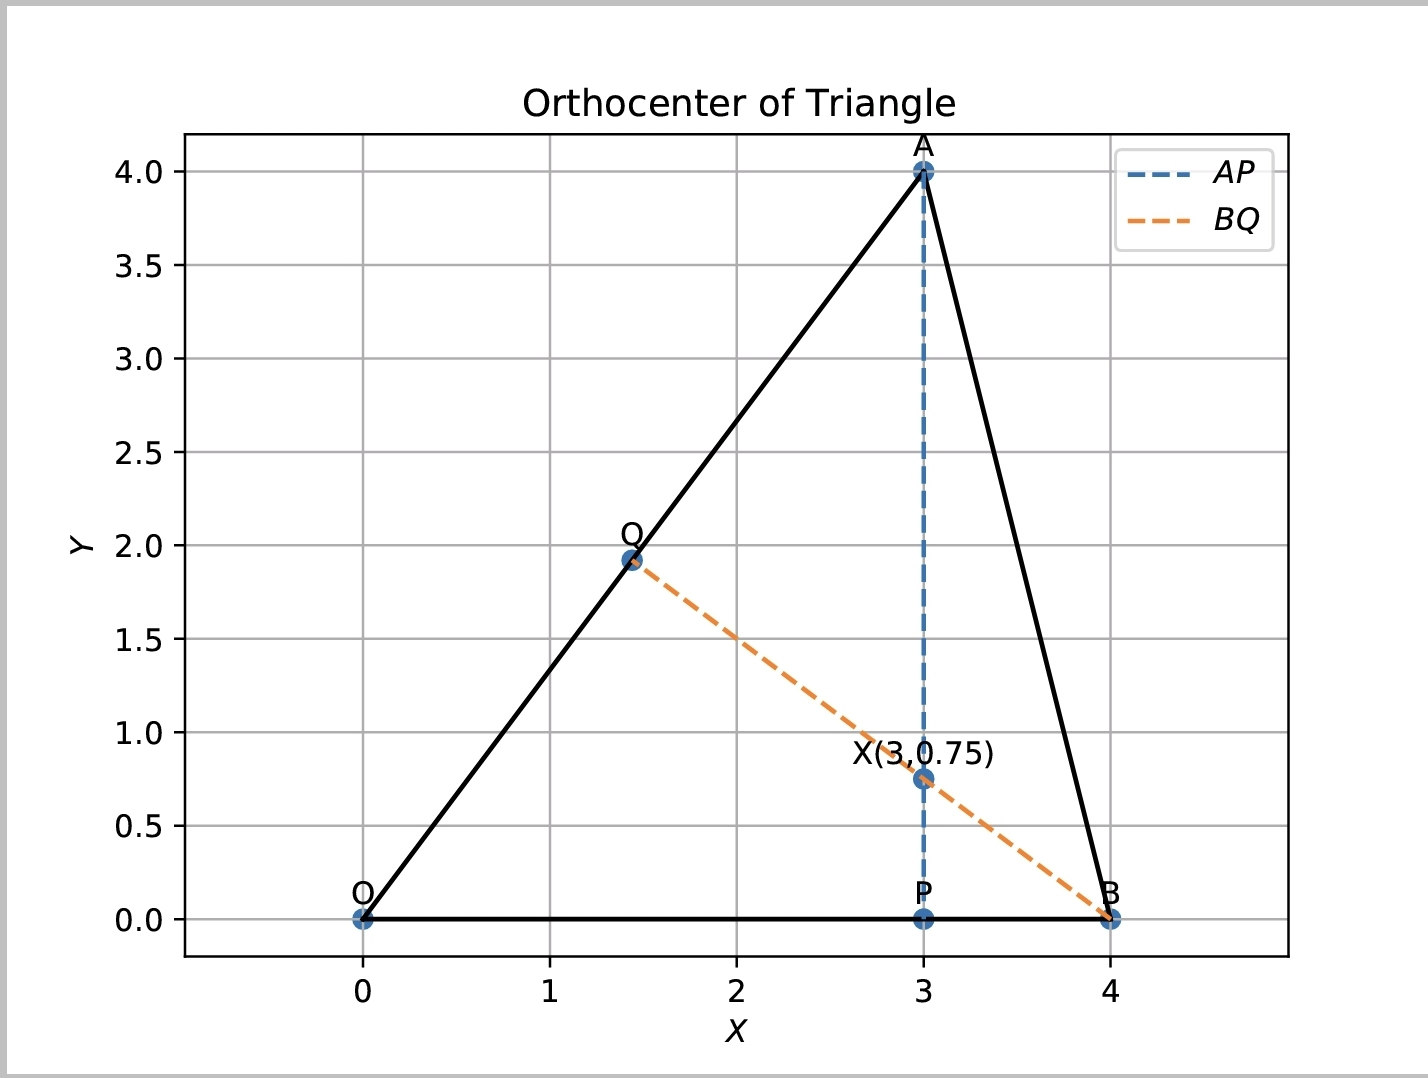
\includegraphics[width=\columnwidth]{fig.jpg}
    \label{fig:my_label}
\end{figure}


\section{\textbf{Code Link}}

\begin{lstlisting}

https://github.com/nikhilnair90/FWC-2/blob/main/Matrix/Conic/conic.py

\end{lstlisting}
Execute the code by using the command\\
\textbf{python3 conic.py}



\end{document}
